% Options for packages loaded elsewhere
\PassOptionsToPackage{unicode}{hyperref}
\PassOptionsToPackage{hyphens}{url}
%
\documentclass[
]{article}
\usepackage{lmodern}
\usepackage{amsmath}
\usepackage{ifxetex,ifluatex}
\ifnum 0\ifxetex 1\fi\ifluatex 1\fi=0 % if pdftex
  \usepackage[T1]{fontenc}
  \usepackage[utf8]{inputenc}
  \usepackage{textcomp} % provide euro and other symbols
  \usepackage{amssymb}
\else % if luatex or xetex
  \usepackage{unicode-math}
  \defaultfontfeatures{Scale=MatchLowercase}
  \defaultfontfeatures[\rmfamily]{Ligatures=TeX,Scale=1}
\fi
% Use upquote if available, for straight quotes in verbatim environments
\IfFileExists{upquote.sty}{\usepackage{upquote}}{}
\IfFileExists{microtype.sty}{% use microtype if available
  \usepackage[]{microtype}
  \UseMicrotypeSet[protrusion]{basicmath} % disable protrusion for tt fonts
}{}
\makeatletter
\@ifundefined{KOMAClassName}{% if non-KOMA class
  \IfFileExists{parskip.sty}{%
    \usepackage{parskip}
  }{% else
    \setlength{\parindent}{0pt}
    \setlength{\parskip}{6pt plus 2pt minus 1pt}}
}{% if KOMA class
  \KOMAoptions{parskip=half}}
\makeatother
\usepackage{xcolor}
\IfFileExists{xurl.sty}{\usepackage{xurl}}{} % add URL line breaks if available
\IfFileExists{bookmark.sty}{\usepackage{bookmark}}{\usepackage{hyperref}}
\hypersetup{
  pdftitle={Sumatriptan versus caffeine for migraine},
  pdfauthor={Andrew J. Sims},
  hidelinks,
  pdfcreator={LaTeX via pandoc}}
\urlstyle{same} % disable monospaced font for URLs
\usepackage[margin=1in]{geometry}
\usepackage{color}
\usepackage{fancyvrb}
\newcommand{\VerbBar}{|}
\newcommand{\VERB}{\Verb[commandchars=\\\{\}]}
\DefineVerbatimEnvironment{Highlighting}{Verbatim}{commandchars=\\\{\}}
% Add ',fontsize=\small' for more characters per line
\usepackage{framed}
\definecolor{shadecolor}{RGB}{248,248,248}
\newenvironment{Shaded}{\begin{snugshade}}{\end{snugshade}}
\newcommand{\AlertTok}[1]{\textcolor[rgb]{0.94,0.16,0.16}{#1}}
\newcommand{\AnnotationTok}[1]{\textcolor[rgb]{0.56,0.35,0.01}{\textbf{\textit{#1}}}}
\newcommand{\AttributeTok}[1]{\textcolor[rgb]{0.77,0.63,0.00}{#1}}
\newcommand{\BaseNTok}[1]{\textcolor[rgb]{0.00,0.00,0.81}{#1}}
\newcommand{\BuiltInTok}[1]{#1}
\newcommand{\CharTok}[1]{\textcolor[rgb]{0.31,0.60,0.02}{#1}}
\newcommand{\CommentTok}[1]{\textcolor[rgb]{0.56,0.35,0.01}{\textit{#1}}}
\newcommand{\CommentVarTok}[1]{\textcolor[rgb]{0.56,0.35,0.01}{\textbf{\textit{#1}}}}
\newcommand{\ConstantTok}[1]{\textcolor[rgb]{0.00,0.00,0.00}{#1}}
\newcommand{\ControlFlowTok}[1]{\textcolor[rgb]{0.13,0.29,0.53}{\textbf{#1}}}
\newcommand{\DataTypeTok}[1]{\textcolor[rgb]{0.13,0.29,0.53}{#1}}
\newcommand{\DecValTok}[1]{\textcolor[rgb]{0.00,0.00,0.81}{#1}}
\newcommand{\DocumentationTok}[1]{\textcolor[rgb]{0.56,0.35,0.01}{\textbf{\textit{#1}}}}
\newcommand{\ErrorTok}[1]{\textcolor[rgb]{0.64,0.00,0.00}{\textbf{#1}}}
\newcommand{\ExtensionTok}[1]{#1}
\newcommand{\FloatTok}[1]{\textcolor[rgb]{0.00,0.00,0.81}{#1}}
\newcommand{\FunctionTok}[1]{\textcolor[rgb]{0.00,0.00,0.00}{#1}}
\newcommand{\ImportTok}[1]{#1}
\newcommand{\InformationTok}[1]{\textcolor[rgb]{0.56,0.35,0.01}{\textbf{\textit{#1}}}}
\newcommand{\KeywordTok}[1]{\textcolor[rgb]{0.13,0.29,0.53}{\textbf{#1}}}
\newcommand{\NormalTok}[1]{#1}
\newcommand{\OperatorTok}[1]{\textcolor[rgb]{0.81,0.36,0.00}{\textbf{#1}}}
\newcommand{\OtherTok}[1]{\textcolor[rgb]{0.56,0.35,0.01}{#1}}
\newcommand{\PreprocessorTok}[1]{\textcolor[rgb]{0.56,0.35,0.01}{\textit{#1}}}
\newcommand{\RegionMarkerTok}[1]{#1}
\newcommand{\SpecialCharTok}[1]{\textcolor[rgb]{0.00,0.00,0.00}{#1}}
\newcommand{\SpecialStringTok}[1]{\textcolor[rgb]{0.31,0.60,0.02}{#1}}
\newcommand{\StringTok}[1]{\textcolor[rgb]{0.31,0.60,0.02}{#1}}
\newcommand{\VariableTok}[1]{\textcolor[rgb]{0.00,0.00,0.00}{#1}}
\newcommand{\VerbatimStringTok}[1]{\textcolor[rgb]{0.31,0.60,0.02}{#1}}
\newcommand{\WarningTok}[1]{\textcolor[rgb]{0.56,0.35,0.01}{\textbf{\textit{#1}}}}
\usepackage{longtable,booktabs}
\usepackage{calc} % for calculating minipage widths
% Correct order of tables after \paragraph or \subparagraph
\usepackage{etoolbox}
\makeatletter
\patchcmd\longtable{\par}{\if@noskipsec\mbox{}\fi\par}{}{}
\makeatother
% Allow footnotes in longtable head/foot
\IfFileExists{footnotehyper.sty}{\usepackage{footnotehyper}}{\usepackage{footnote}}
\makesavenoteenv{longtable}
\usepackage{graphicx}
\makeatletter
\def\maxwidth{\ifdim\Gin@nat@width>\linewidth\linewidth\else\Gin@nat@width\fi}
\def\maxheight{\ifdim\Gin@nat@height>\textheight\textheight\else\Gin@nat@height\fi}
\makeatother
% Scale images if necessary, so that they will not overflow the page
% margins by default, and it is still possible to overwrite the defaults
% using explicit options in \includegraphics[width, height, ...]{}
\setkeys{Gin}{width=\maxwidth,height=\maxheight,keepaspectratio}
% Set default figure placement to htbp
\makeatletter
\def\fps@figure{htbp}
\makeatother
\setlength{\emergencystretch}{3em} % prevent overfull lines
\providecommand{\tightlist}{%
  \setlength{\itemsep}{0pt}\setlength{\parskip}{0pt}}
\setcounter{secnumdepth}{-\maxdimen} % remove section numbering
\ifluatex
  \usepackage{selnolig}  % disable illegal ligatures
\fi
\newlength{\cslhangindent}
\setlength{\cslhangindent}{1.5em}
\newlength{\csllabelwidth}
\setlength{\csllabelwidth}{3em}
\newenvironment{CSLReferences}[2] % #1 hanging-ident, #2 entry spacing
 {% don't indent paragraphs
  \setlength{\parindent}{0pt}
  % turn on hanging indent if param 1 is 1
  \ifodd #1 \everypar{\setlength{\hangindent}{\cslhangindent}}\ignorespaces\fi
  % set entry spacing
  \ifnum #2 > 0
  \setlength{\parskip}{#2\baselineskip}
  \fi
 }%
 {}
\usepackage{calc}
\newcommand{\CSLBlock}[1]{#1\hfill\break}
\newcommand{\CSLLeftMargin}[1]{\parbox[t]{\csllabelwidth}{#1}}
\newcommand{\CSLRightInline}[1]{\parbox[t]{\linewidth - \csllabelwidth}{#1}\break}
\newcommand{\CSLIndent}[1]{\hspace{\cslhangindent}#1}

\title{Sumatriptan versus caffeine for migraine}
\usepackage{etoolbox}
\makeatletter
\providecommand{\subtitle}[1]{% add subtitle to \maketitle
  \apptocmd{\@title}{\par {\large #1 \par}}{}{}
}
\makeatother
\subtitle{A decision tree example}
\author{Andrew J. Sims}
\date{April 2020}

\begin{document}
\maketitle

\hypertarget{introduction}{%
\section{Introduction}\label{introduction}}

This vignette is an example of modelling a decision tree using the
\texttt{rdecision} package. It is based on the example given by Briggs
{[}1, Box 2.3{]} which itself is based on a decision tree which compared
oral Sumatriptan versus oral caffeine/Ergotamine for migraine {[}2{]}.

\hypertarget{creating-the-model}{%
\section{Creating the model}\label{creating-the-model}}

The following code constructs the decision tree. In the formulation used
by \texttt{rdecision}, a decision tree is a form of \emph{arborescence},
a directed graph of nodes and edges, with a single root and a unique
path from the root to each leaf node. Decision trees comprise three
types of node: decision, chance and leaf nodes and two types of edge:
actions (whose sources are decision nodes) and reactions (whose sources
are chance nodes).

\begin{Shaded}
\begin{Highlighting}[]
\CommentTok{\# Time horizon}
\NormalTok{th }\OtherTok{\textless{}{-}} \FunctionTok{as.difftime}\NormalTok{(}\DecValTok{48}\NormalTok{, }\AttributeTok{units=}\StringTok{"hours"}\NormalTok{)}

\CommentTok{\# model variables for cost}
\NormalTok{c.sumatriptan }\OtherTok{\textless{}{-}} \FloatTok{16.10}
\NormalTok{c.caffeine }\OtherTok{\textless{}{-}} \FloatTok{1.32}
\NormalTok{c.ED }\OtherTok{\textless{}{-}} \FloatTok{63.16}
\NormalTok{c.admission }\OtherTok{\textless{}{-}} \DecValTok{1093}

\CommentTok{\# Sumatriptan branch}
\NormalTok{ta }\OtherTok{\textless{}{-}}\NormalTok{ LeafNode}\SpecialCharTok{$}\FunctionTok{new}\NormalTok{(}\StringTok{"A"}\NormalTok{, }\AttributeTok{utility=}\FloatTok{1.0}\NormalTok{, }\AttributeTok{interval=}\NormalTok{th)}
\NormalTok{tb }\OtherTok{\textless{}{-}}\NormalTok{ LeafNode}\SpecialCharTok{$}\FunctionTok{new}\NormalTok{(}\StringTok{"B"}\NormalTok{, }\AttributeTok{utility=}\FloatTok{0.9}\NormalTok{, }\AttributeTok{interval=}\NormalTok{th)}
\NormalTok{c3 }\OtherTok{\textless{}{-}}\NormalTok{ ChanceNode}\SpecialCharTok{$}\FunctionTok{new}\NormalTok{()}
\NormalTok{e1 }\OtherTok{\textless{}{-}}\NormalTok{ Reaction}\SpecialCharTok{$}\FunctionTok{new}\NormalTok{(c3, ta, }\AttributeTok{p=}\FloatTok{0.594}\NormalTok{, }\AttributeTok{label=}\StringTok{"No recurrence"}\NormalTok{)}
\NormalTok{e2 }\OtherTok{\textless{}{-}}\NormalTok{ Reaction}\SpecialCharTok{$}\FunctionTok{new}\NormalTok{(c3, tb, }\AttributeTok{p=}\FloatTok{0.406}\NormalTok{, }\AttributeTok{cost=}\NormalTok{c.sumatriptan, }
                   \AttributeTok{label=}\StringTok{"Relieved 2nd dose"}\NormalTok{)}

\NormalTok{td }\OtherTok{\textless{}{-}}\NormalTok{ LeafNode}\SpecialCharTok{$}\FunctionTok{new}\NormalTok{(}\StringTok{"D"}\NormalTok{, }\AttributeTok{utility=}\FloatTok{0.1}\NormalTok{, }\AttributeTok{interval=}\NormalTok{th)}
\NormalTok{te }\OtherTok{\textless{}{-}}\NormalTok{ LeafNode}\SpecialCharTok{$}\FunctionTok{new}\NormalTok{(}\StringTok{"E"}\NormalTok{, }\AttributeTok{utility=}\SpecialCharTok{{-}}\FloatTok{0.3}\NormalTok{, }\AttributeTok{interval=}\NormalTok{th)}
\NormalTok{c7 }\OtherTok{\textless{}{-}}\NormalTok{ ChanceNode}\SpecialCharTok{$}\FunctionTok{new}\NormalTok{()}
\NormalTok{e3 }\OtherTok{\textless{}{-}}\NormalTok{ Reaction}\SpecialCharTok{$}\FunctionTok{new}\NormalTok{(c7, td, }\AttributeTok{p=}\FloatTok{0.998}\NormalTok{, }\AttributeTok{label=}\StringTok{"Relief"}\NormalTok{)}
\NormalTok{e4 }\OtherTok{\textless{}{-}}\NormalTok{ Reaction}\SpecialCharTok{$}\FunctionTok{new}\NormalTok{(c7, te, }\AttributeTok{p=}\FloatTok{0.002}\NormalTok{, }\AttributeTok{cost=}\NormalTok{c.admission, }\AttributeTok{label=}\StringTok{"Hospitalization"}\NormalTok{)}

\NormalTok{tc }\OtherTok{\textless{}{-}}\NormalTok{ LeafNode}\SpecialCharTok{$}\FunctionTok{new}\NormalTok{(}\StringTok{"C"}\NormalTok{, }\AttributeTok{utility=}\SpecialCharTok{{-}}\FloatTok{0.3}\NormalTok{, }\AttributeTok{interval=}\NormalTok{th)}
\NormalTok{c4 }\OtherTok{\textless{}{-}}\NormalTok{ ChanceNode}\SpecialCharTok{$}\FunctionTok{new}\NormalTok{()}
\NormalTok{e5 }\OtherTok{\textless{}{-}}\NormalTok{ Reaction}\SpecialCharTok{$}\FunctionTok{new}\NormalTok{(c4, tc, }\AttributeTok{p=}\FloatTok{0.920}\NormalTok{, }\AttributeTok{label=}\StringTok{"Endures attack"}\NormalTok{)}
\NormalTok{e6 }\OtherTok{\textless{}{-}}\NormalTok{ Reaction}\SpecialCharTok{$}\FunctionTok{new}\NormalTok{(c4, c7, }\AttributeTok{p=}\FloatTok{0.080}\NormalTok{, }\AttributeTok{cost=}\NormalTok{c.ED, }\AttributeTok{label=}\StringTok{"ED"}\NormalTok{)}

\NormalTok{c1 }\OtherTok{\textless{}{-}}\NormalTok{ ChanceNode}\SpecialCharTok{$}\FunctionTok{new}\NormalTok{()}
\NormalTok{e7 }\OtherTok{\textless{}{-}}\NormalTok{ Reaction}\SpecialCharTok{$}\FunctionTok{new}\NormalTok{(c1, c3, }\AttributeTok{p=}\FloatTok{0.558}\NormalTok{, }\AttributeTok{label=}\StringTok{"Relief"}\NormalTok{)}
\NormalTok{e8 }\OtherTok{\textless{}{-}}\NormalTok{ Reaction}\SpecialCharTok{$}\FunctionTok{new}\NormalTok{(c1, c4, }\AttributeTok{p=}\FloatTok{0.442}\NormalTok{, }\AttributeTok{label=}\StringTok{"No relief"}\NormalTok{)}

\CommentTok{\# Caffeine/Ergotamine branch}
\NormalTok{tf }\OtherTok{\textless{}{-}}\NormalTok{ LeafNode}\SpecialCharTok{$}\FunctionTok{new}\NormalTok{(}\StringTok{"F"}\NormalTok{, }\AttributeTok{utility=}\FloatTok{1.0}\NormalTok{, }\AttributeTok{interval=}\NormalTok{th)}
\NormalTok{tg }\OtherTok{\textless{}{-}}\NormalTok{ LeafNode}\SpecialCharTok{$}\FunctionTok{new}\NormalTok{(}\StringTok{"G"}\NormalTok{, }\AttributeTok{utility=}\FloatTok{0.9}\NormalTok{, }\AttributeTok{interval=}\NormalTok{th)}
\NormalTok{c5 }\OtherTok{\textless{}{-}}\NormalTok{ ChanceNode}\SpecialCharTok{$}\FunctionTok{new}\NormalTok{()}
\NormalTok{e9 }\OtherTok{\textless{}{-}}\NormalTok{ Reaction}\SpecialCharTok{$}\FunctionTok{new}\NormalTok{(c5, tf, }\AttributeTok{p=}\FloatTok{0.703}\NormalTok{, }\AttributeTok{label=}\StringTok{"No recurrence"}\NormalTok{)}
\NormalTok{e10 }\OtherTok{\textless{}{-}}\NormalTok{ Reaction}\SpecialCharTok{$}\FunctionTok{new}\NormalTok{(c5, tg, }\AttributeTok{p=}\FloatTok{0.297}\NormalTok{, }\AttributeTok{cost=}\NormalTok{c.caffeine, }
                    \AttributeTok{label=}\StringTok{"Relieved 2nd dose"}\NormalTok{)}

\NormalTok{ti }\OtherTok{\textless{}{-}}\NormalTok{ LeafNode}\SpecialCharTok{$}\FunctionTok{new}\NormalTok{(}\StringTok{"I"}\NormalTok{, }\AttributeTok{utility=}\FloatTok{0.1}\NormalTok{, }\AttributeTok{interval=}\NormalTok{th)}
\NormalTok{tj }\OtherTok{\textless{}{-}}\NormalTok{ LeafNode}\SpecialCharTok{$}\FunctionTok{new}\NormalTok{(}\StringTok{"J"}\NormalTok{, }\AttributeTok{utility=}\SpecialCharTok{{-}}\FloatTok{0.3}\NormalTok{, }\AttributeTok{interval=}\NormalTok{th)}
\NormalTok{c8 }\OtherTok{\textless{}{-}}\NormalTok{ ChanceNode}\SpecialCharTok{$}\FunctionTok{new}\NormalTok{()}
\NormalTok{e11 }\OtherTok{\textless{}{-}}\NormalTok{ Reaction}\SpecialCharTok{$}\FunctionTok{new}\NormalTok{(c8, ti, }\AttributeTok{p=}\FloatTok{0.998}\NormalTok{, }\AttributeTok{label=}\StringTok{"Relief"}\NormalTok{)}
\NormalTok{e12 }\OtherTok{\textless{}{-}}\NormalTok{ Reaction}\SpecialCharTok{$}\FunctionTok{new}\NormalTok{(c8, tj, }\AttributeTok{p=}\FloatTok{0.002}\NormalTok{, }\AttributeTok{cost=}\NormalTok{c.admission, }\AttributeTok{label=}\StringTok{"Hospitalization"}\NormalTok{)}
 
\NormalTok{th }\OtherTok{\textless{}{-}}\NormalTok{ LeafNode}\SpecialCharTok{$}\FunctionTok{new}\NormalTok{(}\StringTok{"H"}\NormalTok{, }\AttributeTok{utility=}\SpecialCharTok{{-}}\FloatTok{0.3}\NormalTok{, }\AttributeTok{interval=}\NormalTok{th)}
\NormalTok{c6 }\OtherTok{\textless{}{-}}\NormalTok{ ChanceNode}\SpecialCharTok{$}\FunctionTok{new}\NormalTok{()}
\NormalTok{e13 }\OtherTok{\textless{}{-}}\NormalTok{ Reaction}\SpecialCharTok{$}\FunctionTok{new}\NormalTok{(c6, th, }\AttributeTok{p=}\FloatTok{0.920}\NormalTok{, }\AttributeTok{label=}\StringTok{"Endures attack"}\NormalTok{)}
\NormalTok{e14 }\OtherTok{\textless{}{-}}\NormalTok{ Reaction}\SpecialCharTok{$}\FunctionTok{new}\NormalTok{(c6, c8, }\AttributeTok{p=}\FloatTok{0.080}\NormalTok{, }\AttributeTok{cost=}\NormalTok{c.ED, }\AttributeTok{label=}\StringTok{"ED"}\NormalTok{)}

\NormalTok{c2 }\OtherTok{\textless{}{-}}\NormalTok{ ChanceNode}\SpecialCharTok{$}\FunctionTok{new}\NormalTok{()}
\NormalTok{e15 }\OtherTok{\textless{}{-}}\NormalTok{ Reaction}\SpecialCharTok{$}\FunctionTok{new}\NormalTok{(c2, c5, }\AttributeTok{p=}\FloatTok{0.379}\NormalTok{, }\AttributeTok{label=}\StringTok{"Relief"}\NormalTok{)}
\NormalTok{e16 }\OtherTok{\textless{}{-}}\NormalTok{ Reaction}\SpecialCharTok{$}\FunctionTok{new}\NormalTok{(c2, c6, }\AttributeTok{p=}\FloatTok{0.621}\NormalTok{, }\AttributeTok{label=}\StringTok{"No relief"}\NormalTok{)}

\CommentTok{\# decision node}
\NormalTok{d1 }\OtherTok{\textless{}{-}}\NormalTok{ DecisionNode}\SpecialCharTok{$}\FunctionTok{new}\NormalTok{(}\StringTok{"d1"}\NormalTok{)}
\NormalTok{e17 }\OtherTok{\textless{}{-}}\NormalTok{ Action}\SpecialCharTok{$}\FunctionTok{new}\NormalTok{(d1, c1, }\AttributeTok{cost=}\NormalTok{c.sumatriptan, }\AttributeTok{label=}\StringTok{"Sumatriptan"}\NormalTok{)}
\NormalTok{e18 }\OtherTok{\textless{}{-}}\NormalTok{ Action}\SpecialCharTok{$}\FunctionTok{new}\NormalTok{(d1, c2, }\AttributeTok{cost=}\NormalTok{c.caffeine, }\AttributeTok{label=}\StringTok{"Caffeine/Ergotamine"}\NormalTok{)}
 
\CommentTok{\# create lists of nodes and edges}
\NormalTok{V }\OtherTok{\textless{}{-}} \FunctionTok{list}\NormalTok{(}
\NormalTok{  d1, c1, c2, c3, c4, c5, c6, c7, c8,}
\NormalTok{  ta, tb, tc, td, te, tf, tg, th, ti, tj}
\NormalTok{)}
\NormalTok{E }\OtherTok{\textless{}{-}} \FunctionTok{list}\NormalTok{(}
\NormalTok{  e1, e2, e3, e4, e5, e6, e7, e8, e9, e10, e11, e12, e13, e14, e15, e16, }
\NormalTok{  e17, e18}
\NormalTok{)}
\CommentTok{\# tree}
\NormalTok{DT }\OtherTok{\textless{}{-}}\NormalTok{ DecisionTree}\SpecialCharTok{$}\FunctionTok{new}\NormalTok{(V,E)}
\end{Highlighting}
\end{Shaded}

\begin{center}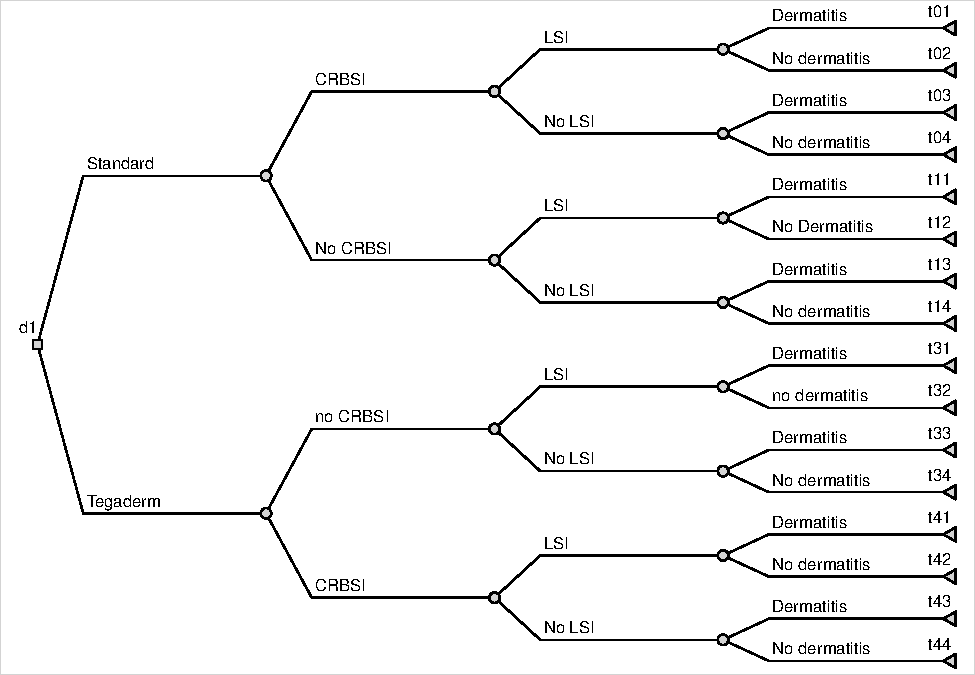
\includegraphics{DT01-Sumatriptan_files/figure-latex/draw-1} \end{center}

\hypertarget{running-the-model}{%
\section{Running the model}\label{running-the-model}}

The method \texttt{evaluate} of decision tree objects computes the
probability, cost and utility of each \emph{strategy} for the model. A
strategy is a unanimous prescription of the actions at each decision
node. In this example there is a single decision node with two actions,
and the strategies are simply the two forms of treatment to be compared.
More complex decision trees are also possible.

The paths traversable in each strategy can be evaluated individually
using the method \texttt{evaluate(by="path")}. In \texttt{rdecision} a
strategy is defined as a set of action edges with one action edge per
decision node. It is necessary to use the option \texttt{by="path"} only
if information about each pathway is required; normally it is sufficient
to call \texttt{evaluate} which will automatically aggregate the
evaluation by strategy.

\hypertarget{model-results}{%
\section{Model results}\label{model-results}}

The evaluation of each pathway, for each strategy, yields the following
table:

\begin{longtable}[]{@{}llrrr@{}}
\toprule
Leaf & d1 & Probability & Cost & Utility\tabularnewline
\midrule
\endhead
A & Sumatriptan & 0.33 & 5.34 & 0.33\tabularnewline
B & Sumatriptan & 0.23 & 7.29 & 0.20\tabularnewline
C & Sumatriptan & 0.41 & 6.55 & -0.12\tabularnewline
D & Sumatriptan & 0.04 & 2.80 & 0.00\tabularnewline
E & Sumatriptan & 0.00 & 0.08 & 0.00\tabularnewline
F & Caffeine/Ergotamine & 0.27 & 0.35 & 0.27\tabularnewline
G & Caffeine/Ergotamine & 0.11 & 0.30 & 0.10\tabularnewline
H & Caffeine/Ergotamine & 0.57 & 0.75 & -0.17\tabularnewline
I & Caffeine/Ergotamine & 0.05 & 3.20 & 0.00\tabularnewline
J & Caffeine/Ergotamine & 0.00 & 0.12 & 0.00\tabularnewline
\bottomrule
\end{longtable}

There are, as expected, ten pathways (5 per strategy). The expected cost
and expected utility for each choice can be calculated from the table
above, or by invoking the \texttt{evaluate} method of a decision tree
object with the default parameter \texttt{by="strategy"}. This gives the
following result, consistent with that reported by Evans \emph{et al}
{[}2{]}.

\begin{longtable}[]{@{}lrr@{}}
\toprule
d1 & Cost & Utility\tabularnewline
\midrule
\endhead
Caffeine/Ergotamine & 4.71 & 0.20128\tabularnewline
Sumatriptan & 22.06 & 0.41686\tabularnewline
\bottomrule
\end{longtable}

\hypertarget{references}{%
\section*{References}\label{references}}
\addcontentsline{toc}{section}{References}

\hypertarget{refs}{}
\begin{CSLReferences}{0}{0}
\leavevmode\hypertarget{ref-briggs2006}{}%
\CSLLeftMargin{1 }
\CSLRightInline{Briggs A, Claxton K, Sculpher M. \emph{Decision
modelling for health economic evaluation}. Oxford, {UK}: : Oxford
University Press 2006. }

\leavevmode\hypertarget{ref-evans1997}{}%
\CSLLeftMargin{2 }
\CSLRightInline{Evans KW, Boan JA, Evans JL, \emph{et al.} Economic
evaluation of oral sumatriptan compared with oral caffeine/ergotamine
for migraine. \emph{Pharmacoeconomics} 1997;\textbf{12}:565--77.}

\end{CSLReferences}

\end{document}
